\documentclass[ ngerman, fontsize= 12pt, paper=a4, headings=big, titlepage=true]{article}

%Sprache
\usepackage{babel}
\usepackage[utf8]{inputenc}
\usepackage[T1]{fontenc}
\usepackage{mathptmx}
\usepackage{hyperref}
\usepackage{lmodern, microtype}
\usepackage{csquotes}
\usepackage{hyperref}
\usepackage{enumerate}

%\usepackage[onehalfspace]{setspace}
%Tablellen:
\usepackage{multirow}
\usepackage{caption}
\usepackage{booktabs}
\usepackage{rotating}
\usepackage{hhline,float}
%\usepackage{pdfpages}

%Mathematik
\usepackage{amsmath}
\usepackage{amsfonts}
\usepackage{amssymb}
\usepackage{mathtools}
\usepackage{bbm}

%Grafik
\usepackage{wrapfig}
\usepackage{color}
\usepackage[svgnames]{xcolor}
\usepackage[
left=3cm,
right=2cm,
top=2.5cm,
bottom=2cm,
%includeheadfoot
]{geometry}

%R-Code
\usepackage{listings}
\lstset{language=R,
	basicstyle=\small\ttfamily,
	stringstyle=\color{DarkGreen},
	otherkeywords={0,1,2,3,4,5,6,7,8,9},
	morekeywords={TRUE,FALSE},
	deletekeywords={data,frame,length,as,character},
	keywordstyle=\color{blue},
	commentstyle=\color{DarkGreen},
}

\begin{document}
	
	
\begin{center}
	\Large
	Technische Universität Dortmund\\
	Fakultät Statistik\\
	Sommersemester 2021\\
	
	\vspace{4em}
	
	Grundlagen der Versuchaplanung: Bericht über das 2.Experiment
	
	\Huge
	\textbf{Temperaturexperiment}
	
	\Large
	\vspace{5em}
	Dozenten:\\
	JProf. Dr. Kirsten Schorning, M.Sc. Onur Gül, B.Sc. Wiebke Dammann\\
	
	
	\vspace{3em}
	Autorinnen: \\
	Kaya Maria Bayer\\
	Ketevan Gurtskaia\\
    Danuscha Große-Hering\\	
	Alicia Hemmersbach\\

	
	
	\vspace{4em}
	
	05.Juli 2021
	
\end{center}

\newpage	

\tableofcontents
\newpage

\section{Einleitung}
Ein Thermometer besitzen vermutlich die meisten Haushalte. Einige davon besitzen wahrscheinlich auch ein Thermometer, welches die Temperatur draußen und drinnen messen kann. Möglicherweise hat man sich bereits die Frage gestellt, worin der Unterschied zwischen dem Innen- und Außensensor dieser Thermometer liegt und ob dieser lediglich darin besteht, dass Außensensoren wetterfest sind, oder ob beide Sensoren unabhängig von weiteren äußeren Einflüssen die gleiche Temperaturen messen würden, wenn man den Innensensor nach außen und den Außensensor nach drinnen legt. \newline 
Genau dieser Frage wird in dem folgenden Temperaturexperiment nachgegangen. Es soll überprüft werden, ob es Unterschiede bei den Messungen der beiden Sensoren drinnen und draußen gibt. \newline
Dazu sollen mit 10 gleichen Thermometern einige Messungen drinnen und draußen durchgeführt werden. Hierbei wird dann der Unterschied der zwei gemessenen Temperaturen zwischen Innen- und Außensensor ausgewertet und mit Hilfe eines statistischen Tests interpretiert. \newline 
Im Folgenden wird auf die Problemstellung des Experiments und die Versuchsbedingungen, dann auf die Analyse des Problems, das zugehörige statistische Modell, die Hypothesen, die statistischen Auswertungsmethoden des Experiment und die Versuchsplanung eingegangen.
\section{Problemstellung und Versuchsbedingungen}
Ziel des Experimentes ist es herauszufinden, ob die Messungen der Innen- und Außensensoren am selben Ort bei gleicher Temperatur übereinstimmen, oder ob es Unterschiede gibt. Außerdem soll untersucht werden, ob es einen Unterschied macht, ob draußen oder drinnen gemessen wird.\newline
Um diese beiden Fragestellungen zu beantworten, sollen insgesamt 3 Messungen mit jeweils 10 Thermometern durchgeführt werden, sodass nach der Durchführung des Experimentes 60 Messwerte vorliegen. Dabei sollen alle Thermometer gleich alt und zudem möglichst neu sein. Außerdem dürfen die Thermometer keine sichtbaren oder bekannten Schäden haben. Die Messungen werden in 3 Zeitslots über einen Tag verteilt ohne extreme Wetterbedingungen vorgenommen, sodass in jedem Zeitslot jeweils eine ähnliche Temperatur vorliegt. Außerdem werden die Thermometer vor jeder Messung randomisiert in 2 Gruppen mit jeweils 5 Thermometern aufgeteilt. Die eine Gruppe der Thermometer misst die Temperatur draußen und die andere Gruppe der Thermometer misst die Temperatur drinnen. Der Raum, in dem drinnen gemessen wird, soll hierbei keine angeschaltete Heizung oder Klimaanlage haben. Außerdem sollen, falls vorhanden, alle Fenster geschlossen sein und derart abgedunkelt, dass keine direkte Sonneneinstrahlung, zum Beispiel durch Fenster, auf die Thermometer trifft. \newline
Die Messungen draußen sollen an einem windgeschützten Ort ohne direkte und auch ohne gespiegelte Sonneneinstrahlung, zum Beisiel durch Wasser, stattfinden. Außerdem sollten die Thermometer an einem trockenen Ort platziert werden und es sollten andere direkte Wärmequellen mindestens 10 Meter Abstand von dem Messort haben. \newline
Für die Messung werden die 5 Thermometer draußen und die 5 Thermometer drinnen jeweils nebeneinander auf einen ebenen identischen Tisch gelegt. Außerdem ist darauf zu achten, dass die Innen- und Außensensoren direkt nebeneinander liegen.  \newline
Die Messungen werden in 3 Zeitslots durchgeführt. Der erste Slot ist von 6:00 - 7:00 Uhr, der zweite von 14:00 - 15:00 Uhr und der dritte Slot von 22:00 - 23:00 Uhr. Insgesamt beträgt jeder Zeitslot eine Stunde und zwischen den Slots liegen jeweils 7 Stunden. Am Abend vor der ersten Messung und nach Ende des ersten und zweiten Zeitslot werden die Thermometer  in den Kühlschrank gelegt. Somit wird die Temperatur von allen Thermometern gleichmäßig neutralisiert. Zu Beginn der drei Zeitslots werden die Thermometer von 2 Versuchsleitern aus dem Kühlschrank geholt und auf den dafür vorgesehenen Tisch gelegt. Dabei ist ein Versuchsleiter für die Thermometer draußen und ein Versuchsleiter für die Thermometer drinnen zuständig. Die Thermometer sollen jeweils 30 Minuten auf dem Tisch liegen und sich der jeweiligen Temperatur anpassen, bevor die 
Temperaturen von den anderen beiden Versuchsleitern abgelesen und notiert werden. Auch hierbei ist ein Versuchsleiter für die Thermometer drinnen und der andere Versuchsleiter für die Thermometer draußen zuständig. Das Ablesen und notieren der Werte soll hierbei möglichst schnell passieren, damit alle 5 Werte jeweils zur gleichen tatsächlich herrschenden Temperatur abgelesen werden. In der möglicherweise verbleibenden Zeit im jeweiligen Zeitslot können die Thermometer jeweils auf den Tischen liegen bleiben, bevor sie dann nach Ablauf des Slots zurück in den Kühlschrank gelegt werden.
\section{Analyse des Problems}
%\begin{enumerate}[-]
%	\item Was ist die interessierende abhängige Variable?
%	Temperaturdifferenz der Innen- und Außensensoren
%	\item Was sind interessierende Einflussvariablen und wie können diese variiert werden? \\
%	\begin{itemize}
%		\item wahre Temperatur (können wir nicht kontrollieren)
%		\item können die Temperatur nicht beeinflussen, können aber die Messzeiten so anpassen, das an dem Messungen unterschiedliche Temperaturen herrschen könnten
%		
%		\item Ort des Thermometers: Drinnen oder Draußen
%	\end{itemize}
%	
%	
%	
%	\item Was sind mögliche Störvariablen und welche können kontrolliert werden?\\
%	Sonne, Wind, Heizung, Klimaanlage/Ventilator, Reaktionszeit, Zustand des Thermometers,  Tageszeit(bezogen auf unterschiedliche Temperaturen am Tag), Thermometer, Luftfeuchtigkeit, Personen im Raum,
%	\item Von welchen Störvariablen soll noch der Einfluss erfasst werden? \\
%	\item Welche Störvariablen sollen als Blockvariablen aufgefasst werden? \\
%	
%	\item die Zeit als Blockvariable (2 Stufen: Morgens/Nachmittags)
%\end{enumerate}

Die vorliegende interessierende Variable ist die Temperaturdifferenz der Innen-und Außensensoren:\\
\begin{center}
	$y_{\text{Differenz}} = y_{\text{AußenSensor}}-y_{\text{Innensensor}} $
\end{center}

Die wahre Temperatur ist eine Einflussvariable. Diese können wir jedoch nicht kontrollieren.  Zudem ist auch der Ort des Thermometers eine interessierende Einflussvariable, welche wir kontrollieren können. In dem Versuch werden wir zwei feste Orte festlegen: Innerhalb und Außerhalb eines Gebäudes. \\

Im folgenden werden mögliche Störvariablen genannt und inwiefern man diese kontrollieren kann. Generell haben die Wetter-bzw. die Klimabedingungen einen hohen Einfluss auf den Versuch.  In geschlossenen Räumen ist dies die Nutzung einer Heizung oder Klimaanlage und die Luftfeuchtigkeit. Die Klimabedingungen im Raum werden Konstant gehalten. Das bedeutet, dass sowohl die Klimaanlage, wie auch die Heizung oder Anlagen zur Regulierung der Luftfeuchtigkeit, ausgeschaltet werden. Außerhalb eines Gebäudes fällt auch die Luftfeuchtigkeit, die Sonnenbestrahlung an dem Messort, die Windstärke, wie auch Regen. Auch diese Bedingungen möchten wir möglichst konstant halten. Dies wird umgesetzt, indem die Thermometer an windgeschützten und überdachten ohne direkter Sonnenbestrahlung platziert werden sollen. Neben diesen Wetterfaktoren, kann auch das Thermometer einen Einfluss haben. Zum einen können Messungenauigkeiten zwischen unterschiedlichen Gererätehersteller oder Modellen zusätzlich zu den Messungenauigkeiten der einzelnen Thermometer dazukommen. Dies würde dazu führen, dass unser Versuch komplizierter würde. Deswegen halten wir das Modell des Thermometers konstant. Zudem ist die Tageszeit bzgl. der unterschiedlichen Temperaaturen am Tage eine Störvariable. Durch die Variation der Messzeiten ist eine Variation der Temperatur möglich. Das bedeutet genauer: Zur Zeit des Sonnenaufgangs ist es tendenziell kälter, als zur Nachmittagszeit.\cite{WK2}. Deswegen wird die Messzeit als Blockvariable mit zwei Stufen aufgefasst. Dabei  entspricht die erste Stufe die Morgenstunden und die zweite Stufe die Nachmittagsstunden. 



\section{Modell, Hypothesen und statistische Auswertungsmethoden}
\section{Versuchsplanung}
\section{Versuchsprotokoll}

\newpage
\textcolor{white}{\section{Literatur}}
\bibliography{Literatur} 
\bibliographystyle{alphadin}
 
 \newpage


\begin{figure}[h]
	\section{Anhang}
	\hspace{-2.3cm}
	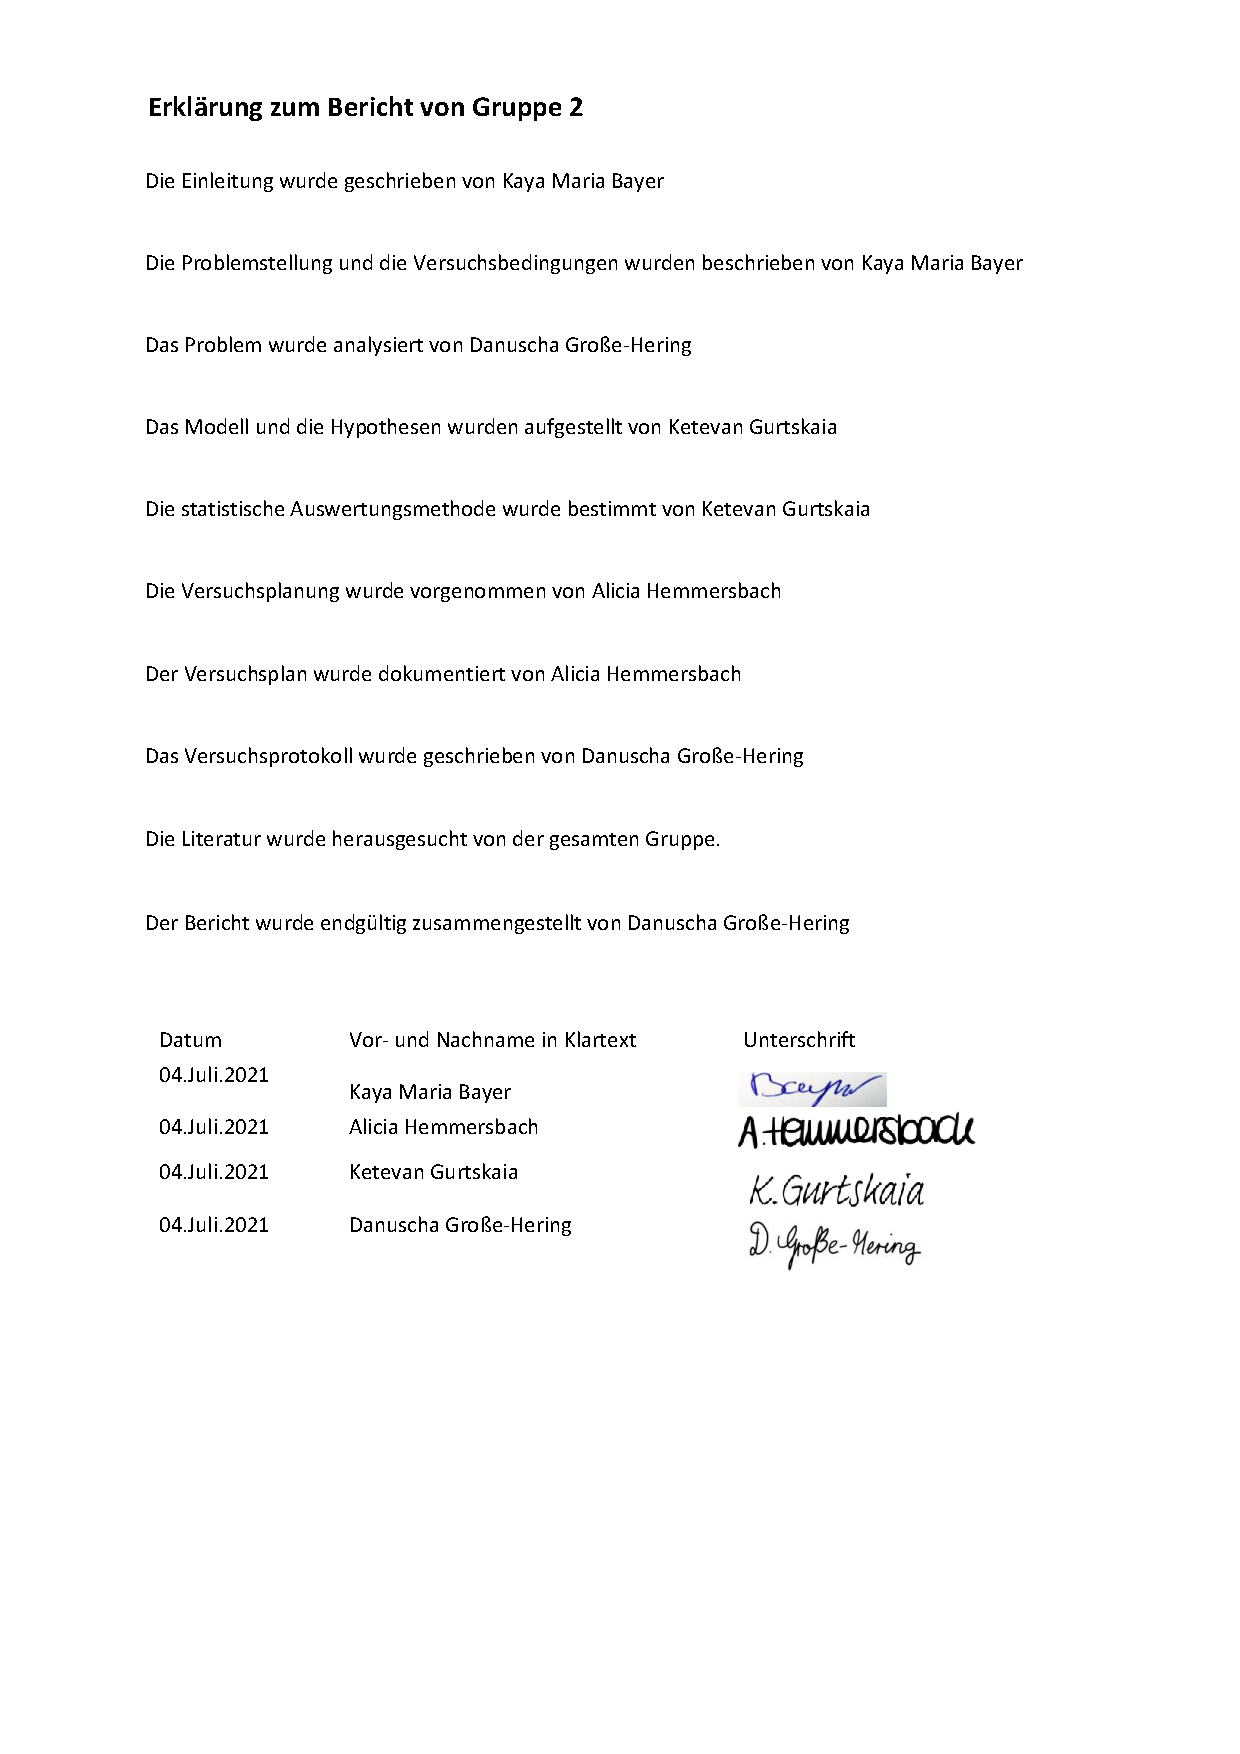
\includegraphics[scale=0.8]{ErklaerungzumBericht}
\end{figure}	

\end{document}


